\documentclass[11pt]{article}
\usepackage{fullpage}
\usepackage{graphicx}
\usepackage{amsmath}
\usepackage{amssymb}
\usepackage{verbatim}
\usepackage{xspace}
\usepackage{tikz}

\begin{document}

\title{Variational IBM Model 1}

\author{}

\maketitle

We want to derive a variational approximation to IBM Model 1 given some bitext $(F, E)$ consisting of $S$ sentence pairs
of French and English text. We will notate that $|F_s| = M_s$ and $|E_s| = N_s$. (Note: the fast\_align paper uses the opposite defitions of $M$ and $N$.)
The model selects for each target word $e_{s,n}$ an
alignment link $a_{s,n}$ in $[1, M_s]$ which indicates that the target word $e$ is generated as a translation of $F_{s,a}$.

This model has two latent variables. The first is the set of alignments $A$, which we will assume have uniform prior over the valid range for each sentence.
The second is $\Phi$, the \emph{translation table}, which gives the translation probability $p(e|f)$ that a source word $f$ generates a target word $e$.
We will assume that each $\phi_f$ is a $|V_E|$-dimensional Dirichlet with parameters ${\alpha_f}_e$, all of which are initially set to $\alpha_0$, a hyperparameter.

A plate diagram of this model is below.

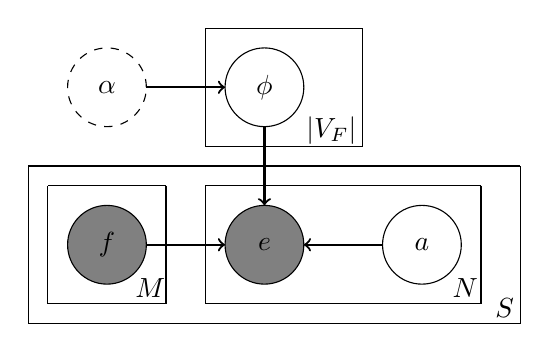
\begin{tikzpicture}
\draw[dashed] (1, 3) circle (0.5cm) node {$\alpha$};
\draw (3, 3) circle (0.5cm) node {$\phi$};
\filldraw[fill=gray] (1, 1) circle (0.5cm) node {$f$};
\filldraw[fill=gray] (3, 1) circle (0.5cm) node {$e$};
\draw (5, 1) circle (0.5cm) node {$a$};

\draw[thick,->] (1.5, 3) -- (2.5, 3);
\draw[thick,->] (1.5, 1) -- (2.5, 1);
\draw[thick,->] (4.5, 1) -- (3.5, 1);
\draw[thick,->] (3, 2.5) -- (3, 1.5);

\draw (0, 0) -- (0, 2);
\draw (0, 2) -- (6.25, 2);
\draw (6.25, 2) -- (6.25, 0);
\draw (6.25, 0) -- (0, 0);
\node[draw=none] at (6.05, 0.2) {$S$};

\draw (0.25, 0.25) -- (0.25, 1.75);
\draw (0.25, 1.75) -- (1.75, 1.75);
\draw (1.75, 1.75) -- (1.75, 0.25);
\draw (1.75, 0.25) -- (0.25, 0.25);
\node[draw=none] at (1.55, 0.45) {$M$};

\draw (2.25, 0.25) -- (2.25, 1.75);
\draw (2.25, 1.75) -- (5.75, 1.75);
\draw (5.75, 1.75) -- (5.75, 0.25);
\draw (5.75, 0.25) -- (2.25, 0.25);
\node[draw=none] at (5.55, 0.45) {$N$};

\draw (2.25, 2.25) -- (2.25, 3.75);
\draw (2.25, 3.75) -- (4.25, 3.75);
\draw (4.25, 3.75) -- (4.25, 2.25);
\draw (4.25, 2.25) -- (2.25, 2.25);
\node[draw=none] at (3.85, 2.45) {$|V_F|$};

\end{tikzpicture}

Mathematically the model is defined as follows. We assume that $F$ and $E$ (and thus their lengths $M$ and $N$) are observed, and that $\alpha$ is given as a hyperparameter.

\begin{align*}
\phi_f &\sim \text{Dir}(|V_E|, \alpha_f)\;\text{for}\;f \in V_F \\
a_{s,n} &\sim \text{Uniform}(1, M_s) \\
e_{s,n} &\sim \text{Categorical}(\phi_{F_{s, a_{s, n}}})
\end{align*}

Recall that $\text{Dir}(\phi | K, \alpha) = \frac{\Gamma(\sum_i\alpha_i)}{\prod_i\Gamma(\alpha)} \prod_{i} \phi_i^{\alpha_i - 1}$.

Thus we can write down the joint probability of the model as
$p(F, E, \Phi, A) = p(\Phi | \alpha) \cdot p(A | F) \cdot p(E | F, A, \Phi)$.
We seek the variational approximation $q(\Phi, A) \approx p(F, E, \Phi, A)$ which we will assume factors as $q(\Phi, A) = q_\Phi(\Phi) \cdot q_A(A)$.

Let's examine the log joint probablity of our model:

\begin{align*}
\ln p(F, E, \Phi, A) &= \ln p(\Phi | \alpha) + \ln p(A | F) + \ln p(E | F, A, \Phi) \\
&= \sum_f \big[ \ln \Gamma(\sum_e {\alpha_f}_e) - \sum_e \ln \Gamma({\alpha_f}_e) + \sum_e ({\alpha_f}_e - 1) \ln {\phi_f}_e \big] \\
&+ \big[\sum_s \sum_{n=1}^{N_s} -\ln M_s \big] \\
&+ \big[ \sum_s \sum_{n=1}^{N_s} \ln {\phi_{F_{s, a_{s, n}}}}_{e_{s,n}} \big] \\
\end{align*}

So if we want $\ln q_A(A) = \mathbb{E}_\Phi \big[ \ln p(F, E, \Phi, A) \big]$ we have:

\begin{align*}
\ln q_A(A) &= \mathbb{E}_\Phi \bigg[ \sum_f \big[ \ln \Gamma(\sum_e {\alpha_f}_e) - \sum_e \ln \Gamma({\alpha_f}_e) + \sum_e ({\alpha_f}_e - 1) \ln {\phi_f}_e \big] \\
&+ \big[\sum_s \sum_{n=1}^{N_s} -\ln M_s \big]\\
&+ \big[ \sum_s \sum_{n=1}^{N_s} \ln {\phi_{F_{s, a_{s, n}}}}_{e_{s,n}} \big] \bigg] \\
&= \mathbb{E}_\Phi \bigg[ \sum_s \sum_{n=1}^{N_s} \ln {\phi_{F_{s, a_{s, n}}}}_{e_{s,n}} \bigg] + C \\
&= \mathbb{E}_\Phi \bigg[ \sum_e \sum_f \text{Count}(e, f) \ln{\phi_f}_e \bigg] + C \\
&= \sum_e \sum_f \text{Count}(e, f) \mathbb{E}_\Phi [\ln {\phi_f}_e] + C \\
\end{align*}

where $\text{Count}(e, f)$ is the number of times the word $e$ is aligned to the word $f$ in the corpus, according to $A$.
According to the wiki page on the Dirichlet Distribution $\mathbb{E}_\Phi [\ln {\phi_f}_e] = \psi({\alpha_f}_e) - \psi(\sum_e {\alpha_f}_e)$ where $\psi$ represents the digamma function.

\begin{align*}
\ln q_A(A) &= \sum_e \sum_f \text{Count}(e, f) \mathbb{E}_\Phi [\ln {\phi_f}_e] + C \\
&= \sum_e \sum_f \text{Count}(e, f) \big(\psi({\alpha_f}_e) - \psi(\sum_e {\alpha_f}_e)\big) + C \\
\end{align*}

Now for $\ln q_\Phi(\Phi) = \mathbb{E}_\Phi \big[ \ln p(F, E, \Phi, A) \big]$ we get:
\begin{align*}
\ln q_\Phi(\Phi) &= \mathbb{E}_A \bigg[ \sum_f \big[ \ln \Gamma(\sum_e {\alpha_f}_e) - \sum_e \ln \Gamma({\alpha_f}_e) + \sum_e ({\alpha_f}_e - 1) \ln {\phi_f}_e \big] \\
&+ \big[\sum_s \sum_{n=1}^{N_s} -\ln M_s \big]\\
&+ \big[ \sum_s \sum_{n=1}^{N_s} \ln {\phi_{F_{s, a_{s, n}}}}_{e_{s,n}} \big] \bigg] \\
&= \mathbb{E}_A \bigg[ \big[ \sum_f \sum_e ({\alpha_f}_e - 1) \ln {\phi_f}_e \big] + \big[ \sum_s \sum_{n=1}^{N_s} \ln {\phi_{F_{s, a_{s, n}}}}_{e_{s,n}} \big] \bigg] + C \\
&= \mathbb{E}_A \bigg[ \big[ \sum_f \sum_e ({\alpha_f}_e - 1) \ln {\phi_f}_e \big] + \big[ \sum_e \sum_f \text{Count}(e, f) \ln {\phi_f}_e \big] \bigg] + C \\
&= \sum_f \sum_e ({\alpha_f}_e - 1) \ln {\phi_f}_e + \mathbb{E}_A \bigg[ \sum_e \sum_f \text{Count}(e, f) \ln {\phi_f}_e \bigg] + C \\
&= \sum_f \sum_e ({\alpha_f}_e - 1) \ln {\phi_f}_e + \sum_e \sum_f \mathbb{E}_A\big[\text{Count}(e, f)\big] \ln {\phi_f}_e + C \\
&= \sum_f \sum_e \bigg({\alpha_f}_e + \mathbb{E}_A\big[\text{Count}(e, f)\big] - 1\bigg) \ln {\phi_f}_e + C \\
\end{align*}

From this it's clear that each $\phi_f$ is now a non-symmetric Dirichlet with parameters $\alpha_0 + \mathbb{E}_A[\text{Count}(e, f)]$ for each $e \in V_e$.

This suggests the following simple algorithm for model 1:

\begin{enumerate}
\item Initialize $\alpha_{f,e}$ to $\alpha_0$ $\forall f, e$
\item For each iteration:
\item Initialize $\alpha' = \alpha$
\item Loop over $s$ and $n$. Let $e = E_{s,n}$. For each source word $f \in F_s$ add $\psi({\alpha_f}_e) - \psi(\sum_{e' \in E_s} {\alpha_f}_e')$ to $\alpha'_{f,e}$.
\item Update $\alpha = \alpha'$
\item Repeat until convergence 
\end{enumerate}

See variational\_ibm1.py for an implementation of this algorithm.
\end{document}
